\documentclass{article}
\usepackage[utf8]{inputenc}
\usepackage{graphicx}

\author{Bijan Varjavand}
\title{LabNotebook}
\date{April 25, 2017}

\begin{document}

\maketitle

\section{Objectives}

The objective for our group this day was to use the transistors we created and measure their outputs and properties.

\section{Setup}

Different students were available for this lab which worked in Professor Katz's lab. They were available to guide us and were able to bring us to their space in their lab so we could use their tools.

\subsection{Materials}

The two materials we used for our transistors were PQT-12 and ZTO. The class of transistor these materials make is that of a MOSFET. We had silicon squares prepared as a semiconductor.

\subsection{Tools}

The tools we used were the different pieces of equipment in Katz's lab.

\section{Procedure}

We followed the instructions of the TA. They did not spend much time explaining their procedure so some of the process is still unknown.

\section{Results}

The curves we got from our ZTO transistor is shown below. We were unable to make the PQT-12 transistor work, maybe due to contamination (which spin coating is susceptible to).

\begin{figure}[h!]
\centering
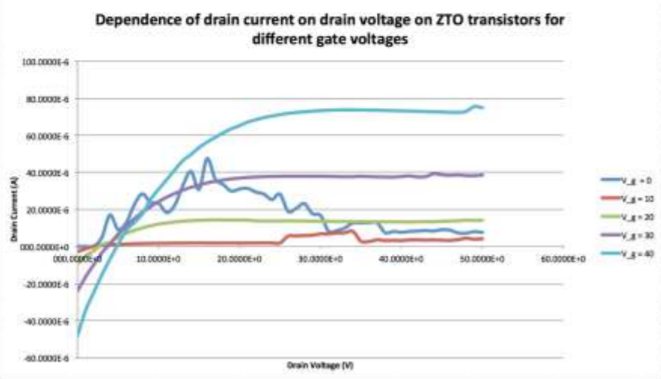
\includegraphics[scale=0.8]{trans.png}
\end{figure}

\section{Observations}

We saw that current increases exponentially as voltage increases, until saturation current is reached. Current approaches a space-charge limited region which causes it to stop increasing significantly. The error in our data is from the curve with 0 gate voltage - a special case which is prone to errors. It should ideally have been a flat line.

\end{document}